
\label{chap-gds}


\section{Introduction}

The previous chapter makes clear that we face a trade-off in using \mdsap. If the ordering of the points in space is to be maintained, a sufficiently high dimensional projection of the data must be obtained. But increasing the projection dimension causes the nullspace of the penalty to become large, causing a large space of wiggly functions to be used without being penalised, leading to unreliable smoothing results. 

The requirement we seek is clear: we wish to smooth in as many dimensions as possible; but while doing this we must also limit the nullspace of the penalty. Fortunately, this is possible using the ideas put forth in \cite{duchon77}. The methods detailed there give a generalisation of the thin plate spline that allows for a smaller nullspace to be used.

The next section goes into the technical detail of how this approach works. Section \ref{gds-wad-examples} shows how this can be useful in the within-area distance case discussed in chapters \label{chap-sc} and \label{chap-mds}. Section \ref{gds-gds-examples} gives examples of generalized distance smoothing.

\section{From thin plate splines to Duchon splines}

\cite{simonbook} p. 153 gives the formulation for the thin plate penalty in $d$ dimensions with penalty order $m$ as:
\begin{equation}
J_{m,d} = \int \ldots \int_{\mathbb{R}^n} \sum_{\nu_1 + \dots + \nu_d=m} \frac{m!}{\nu_1! \dots \nu_d!}\Big( \frac{\partial^m f(x_1,\dots,x_d)}{\partial x_1^{\nu_1} \ldots  \partial x_d^{\nu_d}} \Big)^2 \text{d} x_1 \ldots  \text{d} x_d,
\label{tprs-pen}
\end{equation}
where the summation index generates all of the possible combinations of penalty orders such than their sum is still $m$ (thereby finding all the correct cross-terms). The technical restriction $2m>d$ is also imposed to ensure that $f$ remains continuous.

The form of $f$ is:
\begin{equation}
f(\mathbf{x}) = \sum_{i=1}^n \delta_i \eta_{md}(\mathbf{x}-\mathbf{x_i}) + \sum_{j=1}^M \alpha_j \phi_j(\mathbf{x}),
\label{tprs-basis}
\end{equation}
(\cite{wood2003}) where the first summation is a series of radial basis functions, one per datum and the second sums the unpenalised terms in the nullspace of the penalty. These are $M$ linearly independent polynomials of degree less than $m$. $M$ is given by:
\begin{equation*}
M=\begin{pmatrix} m+d-1 \\ d  \end{pmatrix}.
\end{equation*}
In the cases presented so far, $d$ (the MDS projection dimension) is known and $m$ is dictated by $d$. Increasing $d$ increases $m$ (by the continuity condition that $2m>d$) and hence increases $M$ in the manner above. Therefore $M$ increases very quickly with the number of dimensions used; this is shown in figure \ref{nullspace-dim} (blue line). As more functions are included in the nullspace, the more and more complex (because of their linear independence) the functions are. Having very wiggly functions in the nullspace is certainly undesirable, having many of them will be extremely problematic for model parsimony. 

\begin{figure}
\centering
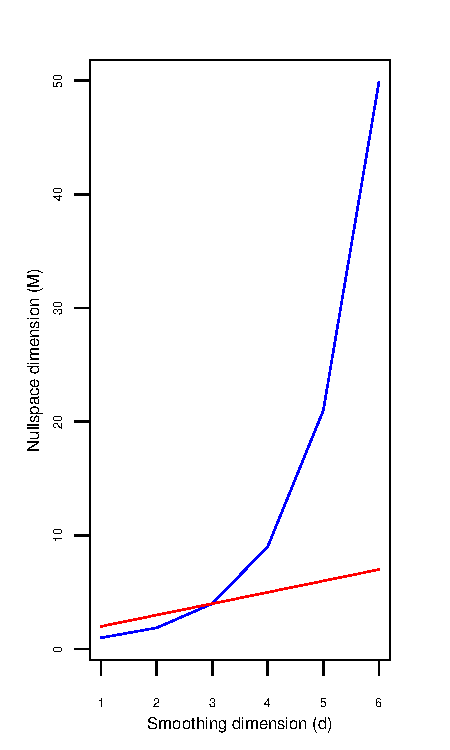
\includegraphics[width=3in]{gds/figs/nullspace-dim.pdf} \\
\caption{Relationship between smoothing dimension ($d$) and the nullspace dimension ($M$) for thin plate regression splines (blue) and Duchon splines (red).}
\label{nullspace-dim}
% generated by thesis/mds/figs/nullspace-dim.R
\end{figure}

A top-down rigorous proof and treatment of Duchon splines is given in \cite{duchon77}; below is an informal explanation of how from (\ref{tprs-pen}) one can reach the penalty given by Duchon. 

The usual thin plate regression spline penalty given in (\ref{tprs-pen}) can be thought of as a measure of ``wigglyness'' or ``roughness'', taking higher values when $f$ is particularly rough or wiggly (the penalty prevents the spline from interpolating). Integrating the square of the derivatives over the whole of $\mathbb{R}^d$ allows us to consider the GAM fitting procedure as minimizing the objective function in such a way that reduces the wigglyness across the whole of $f$ whilst being as close to the data as possible. 

\cite{duchon77} proposes a penalty that is more general than (\ref{tprs-pen}), the first step from (\ref{tprs-pen}) is to consider taking the Fourier transform of the derivatives before squaring and integrating them. The Fourier transform allows us to consider the penalty as an infinite sum of frequencies; decomposing functions defined in space into their frequency domain representations. Mathematically, the Fourier transform of some function of $d$-dimensional space ($\mathbf{x}$), $g$, is defined as:
\begin{equation*}
\mathfrak{F} g(\boldsymbol{\tau}) = \int \ldots \int_{\mathbb{R}^d} e^{2 \pi \sqrt{-1} \mathbf{x}^\text{T} \boldsymbol{\tau}} g(\mathbf{x}) \text{d}\mathbf{x}.
\end{equation*}
Here $\mathfrak{F}$ is an operator applied to $g$, so $\mathfrak{F}g$ may be considered as a function of $\boldsymbol{\tau}$ (a $d$-vector of continuous frequency spectra). More detail on Fourier transforms can be found in (for example) \cite{bracewell}, \cite{chu-ft} and \cite{beerends}. 

Taking the Fourier transform of the penalty allows us to think of how the penalty is calculated in a different way. Rather than thinking about measuring the wigglyness over the whole of $f$, point by point, instead the measure is based on the frequencies of $f$, the higher the frequency components contribute more to the integral than the lower ones. Intuitively this makes sense, since the low frequency components of $f$ are likely performing a similar task to those functions in the nullspace of the penalty, where as the more complicated, high frequency components are more likely to represent $f$ attempting to interpolate parts of the smooth where consecutive dissimilar values occur.

Taking the Fourier transform of the derivative terms in (\ref{tprs-pen}) yields the following penalty:
\begin{equation}
J_{m,d} = \int \ldots \int_{\mathbb{R}^d} \sum_{\nu_1 + \dots + \nu_d=m} \frac{m!}{\nu_1! \dots \nu_d!}\Big( \mathfrak{F} \frac{\partial^m f}{\partial x_1^{\nu_1} \ldots  \partial x_d^{\nu_d}}(\boldsymbol{\tau}) \Big)^2 \text{d} \boldsymbol{\tau}.
\label{tprs-pen-ft}
\end{equation}
The penalties (\ref{tprs-pen}) and (\ref{tprs-pen-ft}) are in fact equivalent by Plancherel's theorem (\cite{vretblad} p. 180), so one can take either view and obtain the same numerical value for the penalty. 

We could extend this frequency-based interpretation of the penalty to a more general class of penalties by putting a weighting in the integral:
\begin{equation}
\int \ldots \int_{\mathbb{R}^d} w(\boldsymbol{\tau}) \sum_{\nu_1 + \dots + \nu_d=m} \frac{m!}{\nu_1! \dots \nu_d!}\Big( \mathfrak{F} \frac{\partial^m f}{\partial x_1^{\nu_1} \ldots  \partial x_d^{\nu_d}}(\boldsymbol{\tau}) \Big)^2 \text{d} \boldsymbol{\tau},
\label{duchon-penalty-general}
\end{equation}
the function $w$ could then be used to pick out particularly high frequencies and penalise those more than the lower frequency ones. Setting $w(\boldsymbol{\tau})=1, \forall \boldsymbol{\tau}$ allows us to recover (\ref{tprs-pen}).

Duchon shows that if $w(\boldsymbol{\tau})= \lvert \boldsymbol{\tau} \rvert^{2s}$ is used then the thin plate spline functions in (\ref{tprs-basis}) arise. In this case the above penalty becomes:
\begin{equation}
\breve{J}_{m,d} = \int \ldots \int_{\mathbb{R}^d} \lvert \boldsymbol{\tau} \rvert^{2s} \sum_{\nu_1 + \dots + \nu_d=m} \frac{m!}{\nu_1! \dots \nu_d!}\Big( \mathfrak{F} \frac{\partial^m f}{\partial x_1^{\nu_1} \ldots  \partial x_d^{\nu_d}}(\boldsymbol{\tau}) \Big)^2 \text{d} \boldsymbol{\tau}.
\label{duchon-penalty}
\end{equation}
Again, (\ref{tprs-pen}) can be recovered from this penalty (by setting $s=0$). When $s>0$ higher frequencies are penalised more than lower ones. In order to obtain smooth functions it is required that $m+s>d/2$. So $s$ can be used to allow high dimensional smoothing, while still using lower-order penalties without yielding discontinuous functions. One can therefore think of $s$ as a kind of ``fudge factor'' that allows the conditions on $m$ and $d$ to be relaxed; given some fixed combination of $m$ and $d$, an $s$ can be found (by simply calculating $s=d/2-m$).

Looking back to figure \ref{nullspace-dim} (where the blue line showed the increasing numbers of functions in the nullspace of the conventional thin plate penalty), the red line gives the number of functions in penalty (\ref{duchon-penalty}). In this case $m=2$ has been chosen to remain constant as the dimensionality increases, leading to a linear increase in nullspace size with the smoothing dimension.

\textbf{SIMON} : If I can construct some kind of proof that the MDS projection of within-area distances always leads to a manifold then I'll say something here about how that leads to the following \ldots In any small region a 2-dimensional manifold will look like $\mathbb{R}^2$, in the same small region the smoother's behaviour will closely approximate a regular thin plate regression spline with $m=2$ on the tangent space of the manifold (as the smoothing parameter tends to zero, at least).

\cite{girosi} discusses the connections between neural networks and GAMs with the more general form of this type of penalty (ie. (\ref{duchon-penalty-general})) (see also \cite{elements} p. 168).


\subsection{Duchon splines with \mdsap\ -- \mdsds}

With the addition of Duchon splines to the \mdsap\ we are now in a position to project data into any number of dimensions and smooth over the response without having to worry about the nullspace of the penalty causing problems.










\section{Choosing MDS projection dimension}

With Duchon's basis in mind, it is now possible to smooth a space of any dimension using a second order derivative penalty, simply by picking $s$ appropriately. Picking the dimension of the MDS projection is now a concern since there is no reason to believe that simply going to higher and higher dimensions will yield better and better results. Keeping in mind the desire for a parsimony, it would be preferable to keep the dimension of the projection as small as possible.

\subsection{Using proportion of variation explained}

It is clear that as higher and higher projections are used, a larger and larger proportion of the variation in the distance matrix is explained. It therefore seems reasonable to base the choice of dimension on the proportion of the variation explained in the initial grid. However, what proportion should be used? 80\%? 90\%? 99\%? There is no reason to choose any one of these over the others. Setting the proportion of variation to be explained generally is surely a bad idea, since what works for one domain may well be a disaster for another.

\subsection{Using scores}

Since fitting a GAM with a Duchon spline basis is relatively cheap compared to the cost of finding the within-area distances, the GCV score can be used to find an optimal dimension for the MDS projection. So, using this to our advantage, a series of projections can be tried, their GCV scores calculated, and the best selected as the projection to use for the model.

In particular, starting from a 2-dimensional projection, the dimensionality is increased  and models fitted, until there is an increase in GCV score. The upper bound is the number of dimensions that explain 95\% of the variation in the distance matrix of the initial grid (see section \ref{grids}).  This favours simpler models (in dimensionality terms), although of course a full search can be performed if there is some prior belief that the dimensionality should be higher (indeed there is no reason to believe that the GCV score should be unimodal in dimension). It might be considered preferable to take the first minima in the score anyway as we ould generally prefer a simpler model. Simulations show that the minima in the GCV score and MSE are in agreement.

Figure \ref{wt2-gcv-projdim-boxplot} shows a plot of GCV score and mean squared error for 60 simulations from the peninsula domain, for each of the 60 realisations a \mdsds\ was fitted using a 2 through 20 dimensional projection. The boxplots are grouped according to the dimension of the MDS projection used. The graph shows that there is a minima in the score when the dimension is four which corresponds with the minimum MSE.

\begin{figure}
\centering
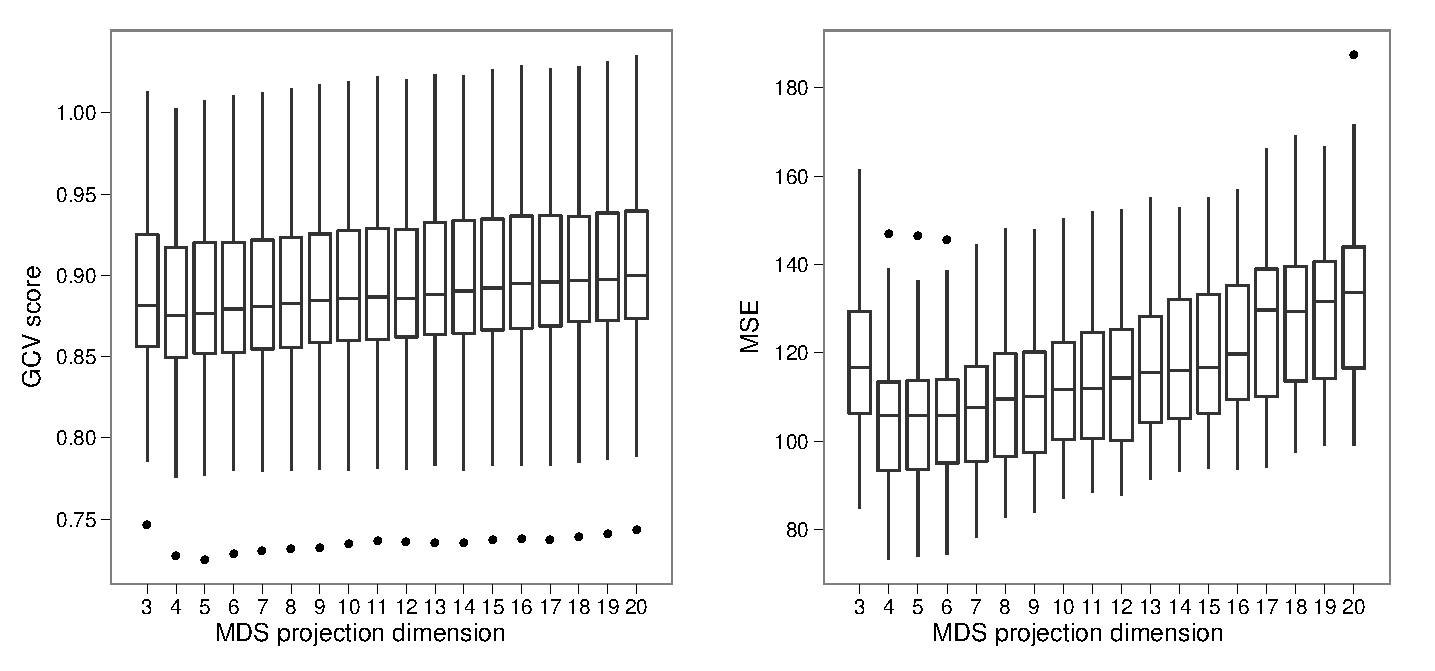
\includegraphics[width=6in]{mds/figs/wt2-gcv-projdim-boxplot.pdf} \\
\caption{MSE and GCV score for the peninsula domain when different dimensional projections are used. Here a 4-dimensional projection gives a minimum GCV score and MSE.}
\label{wt2-gcv-projdim-boxplot}
% generated by mds/duchon/wt2-gcvml.R
\end{figure}

The ML score (\cite{remlpaper}), can be adapted into an AIC-like score to be used in place of the GCV score, provided there is appropriate penalisation to take into account the increase in the dimension of the projection space. Following score was used:
\begin{equation*}
\text{ML}_p = -2 \hat{l} + 2P
\end{equation*}
where $\hat{l}$ is the log-likelihood at the MLE and $P$ is a penalty which is the nullspace dimension (ie. $M$ from above with $m=2$ and $d$ set to the MDS projection dimension):
\begin{align*}
P =& \begin{pmatrix} 2+d-1 \\ d  \end{pmatrix},\\
=& \begin{pmatrix} d+1 \\ d  \end{pmatrix},\\
=& d+1.
\end{align*}
So the score used to select dimension is:
\begin{equation*}
\text{ML}_p = -2 \hat{l} + 2(d+1)
\end{equation*}
Since the maximum basis is kept constant, but the dimension of the problem changes, this penalty attempts to stop small increases in the likelihood by increasing dimension. This allows the ML score to be used to fit each individual GAM and then comparisons to be made between models of different dimensions. Note the similarity to the AIC.

There is, of course, no guarantee that there will always be a minimum to find and as with all automated methods, practitioners should be mindfull of what could potentially go wrong. However, in the situations tested (see below for examples), both of these methods appeared to be satisfactory.

\section{Within-area distance examples}
\label{gds-wad-examples}
\subsection{Simulations}

Returning to the simulation study in section \ref{wt2bigsim}, the same set of simulations (250 samples at three error levels) was re-run but now using the Duchon splines, selecting MDS dimension based on both GCV and $\text{ML}_p$ scores (maximum spline basis dimension was set at 100). The results are shown for the original simulations (for thin plate splines and the soap film smoother) along side those for the new model.

Figure \ref{wt2-boxplot-duchon} shows the boxplots for these simulations, \mdsds\ with GCV dimension selection does better than the soap film smoother when the noise is low and was indistinguishable (via a paired Wilcoxon signed rank test) from the soap film smoother at higher noise levels. Using $\text{ML}_p$ gave roughly similar results, becoming significantly different from the soap film smoother at high noise levels.

\begin{figure}
\centering
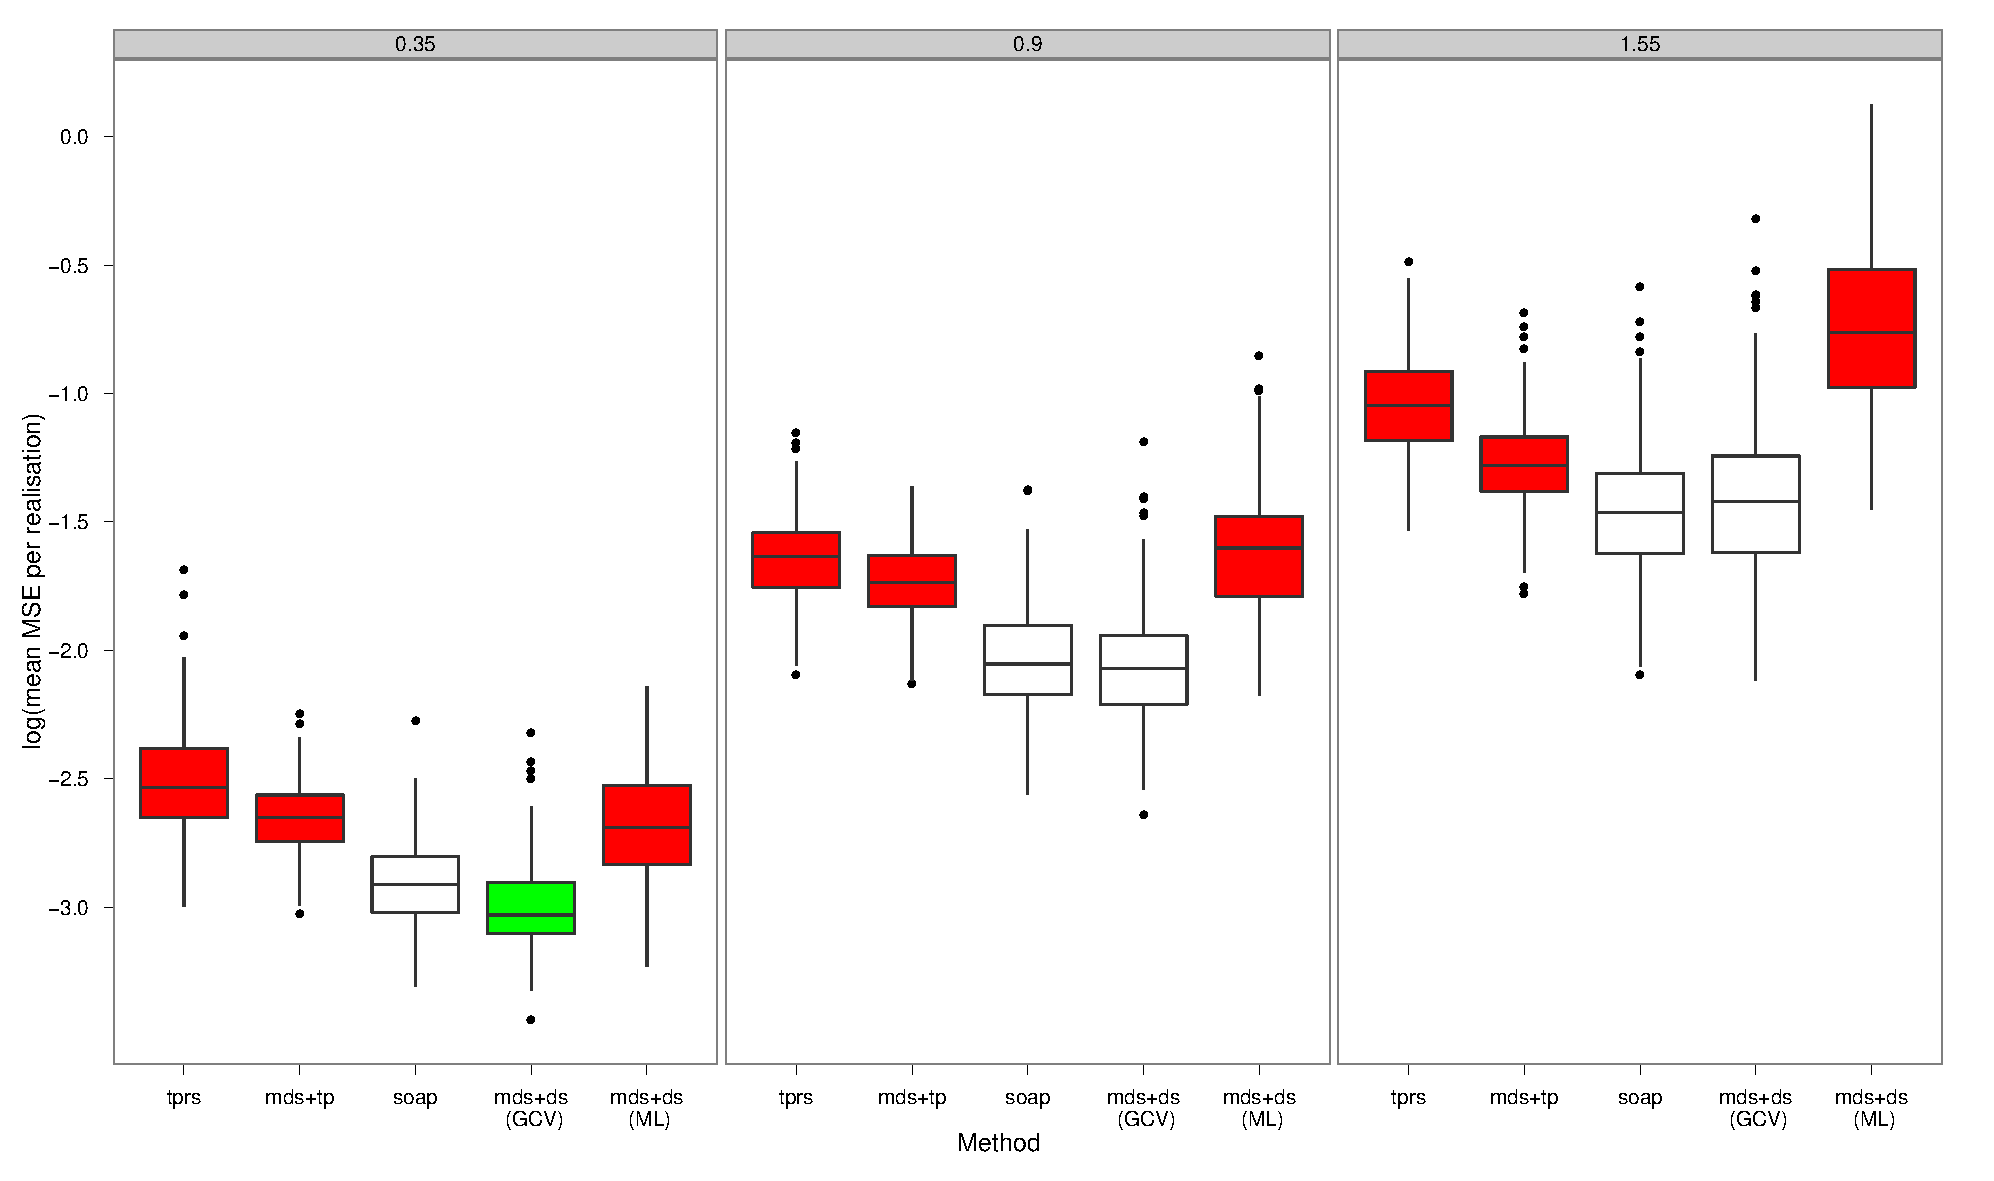
\includegraphics[width=6in]{mds/figs/wt2-boxplot-duchon.pdf} \\
\caption{Boxplots of logarithm of per realisation average mean squared error from simulations on the peninsula domain. The boxplots are in groups of four for each error level $(\sigma = 0.35, 0.9, 1.55)$. Colours indicate the result of a Wilcoxon paired signed rank test of whether the MSE was significantly (p$<10^{-2}$) different from the soap film smoother. Red indicates different and worse, green different and better.}
\label{wt2-boxplot-duchon}
% generated by mds/duchon/bigsim/boxplot-wt2.R
\end{figure}

\textbf{SIMON}: do you think I should put some more examples in here? Perhaps a new set of simulations (based on the ``comb'' in section 3.7.2, fig 3-24)?

\subsection{Revisiting the Aral sea}

Going back to the Aral sea example from section \ref{aral-sec}, we can fit a model using the optimal (in a GCV score sense) dimension. Figure \ref{mds-aral-5d-duchon} shows the raw data and a smoothed version, using a 5-dimensional projection (given by minimising the GCV score). The plot does not contain any of the artefacts that were present in the previous smooths of the data.

\begin{figure}
\centering
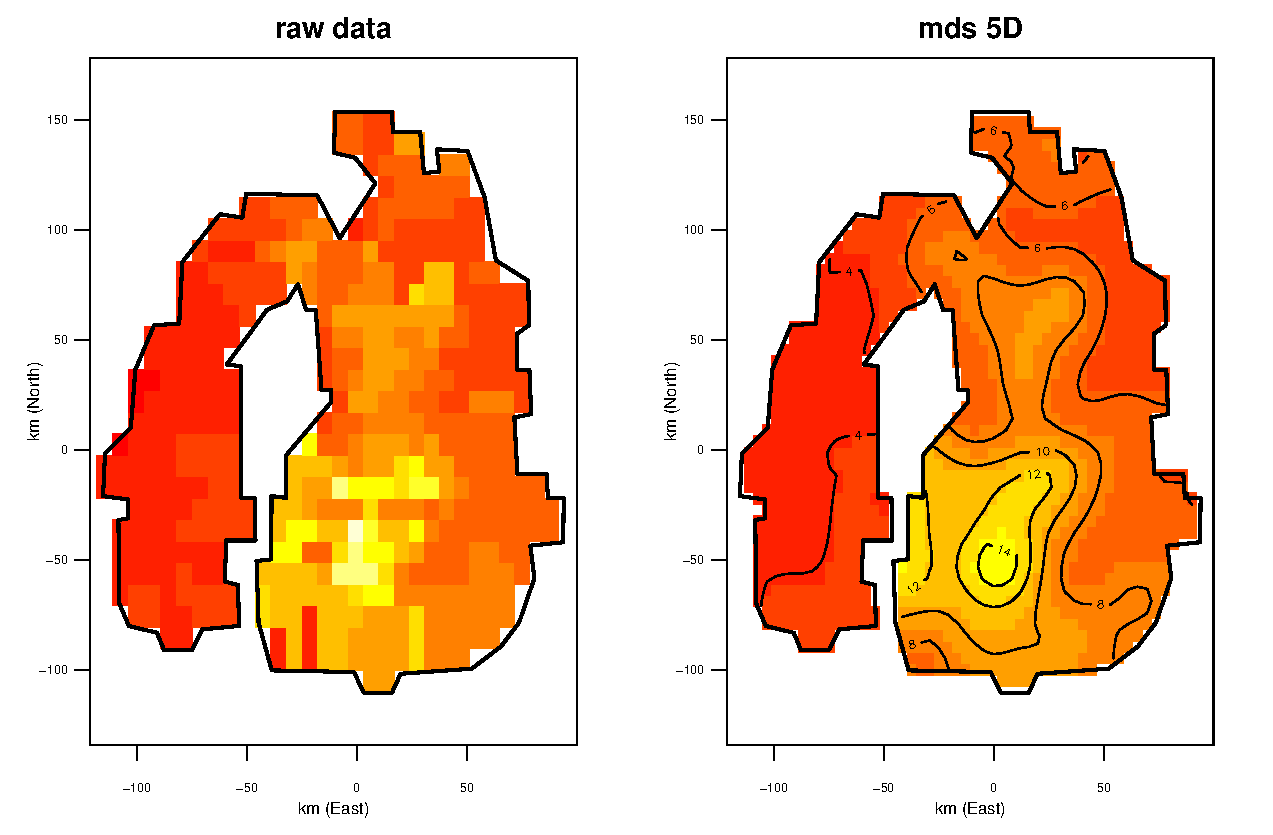
\includegraphics[width=6in]{mds/figs/aral-5d-duchon.pdf} \\
\caption{The Aral sea chlorophyl levels smoothed using Duchon splines, when a 5-dimensional MDS projection is employed. Note the lack of artefacts in comparison to previous \mdsap\ models.}
\label{mds-aral-5d-duchon}
% generated by duchon/aral-evolve.R
\end{figure}

Using the $\text{ML}_p$ statistic to select the MDS projection dimension resulted in a 19 dimensional smooth. While the 

Figure \ref{gds-aral-dim-select} shows plots of score (both GCV and $\text{ML}_p$) against MDS projection dimension. The GCV plot shows a clear minima where as $\text{ML}_p$ does not.


\begin{figure}
\centering
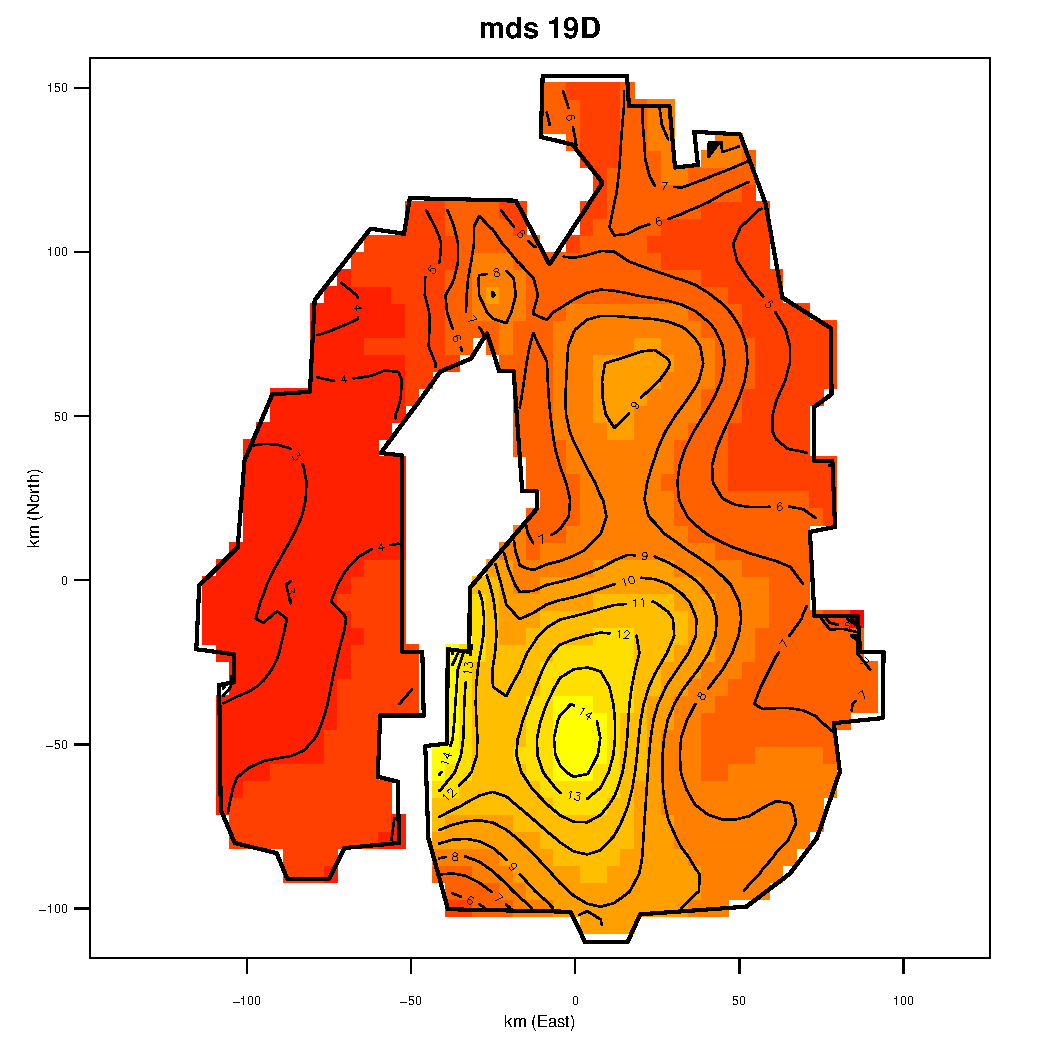
\includegraphics[width=6in]{gds/figs/aral-19d.pdf} \\
\caption{TKTKTK caption}
\label{gds-aral-19d}
% generated by duchon/aral-scoreplots.R with liberal use of commenting
\end{figure}


\begin{figure}
\centering
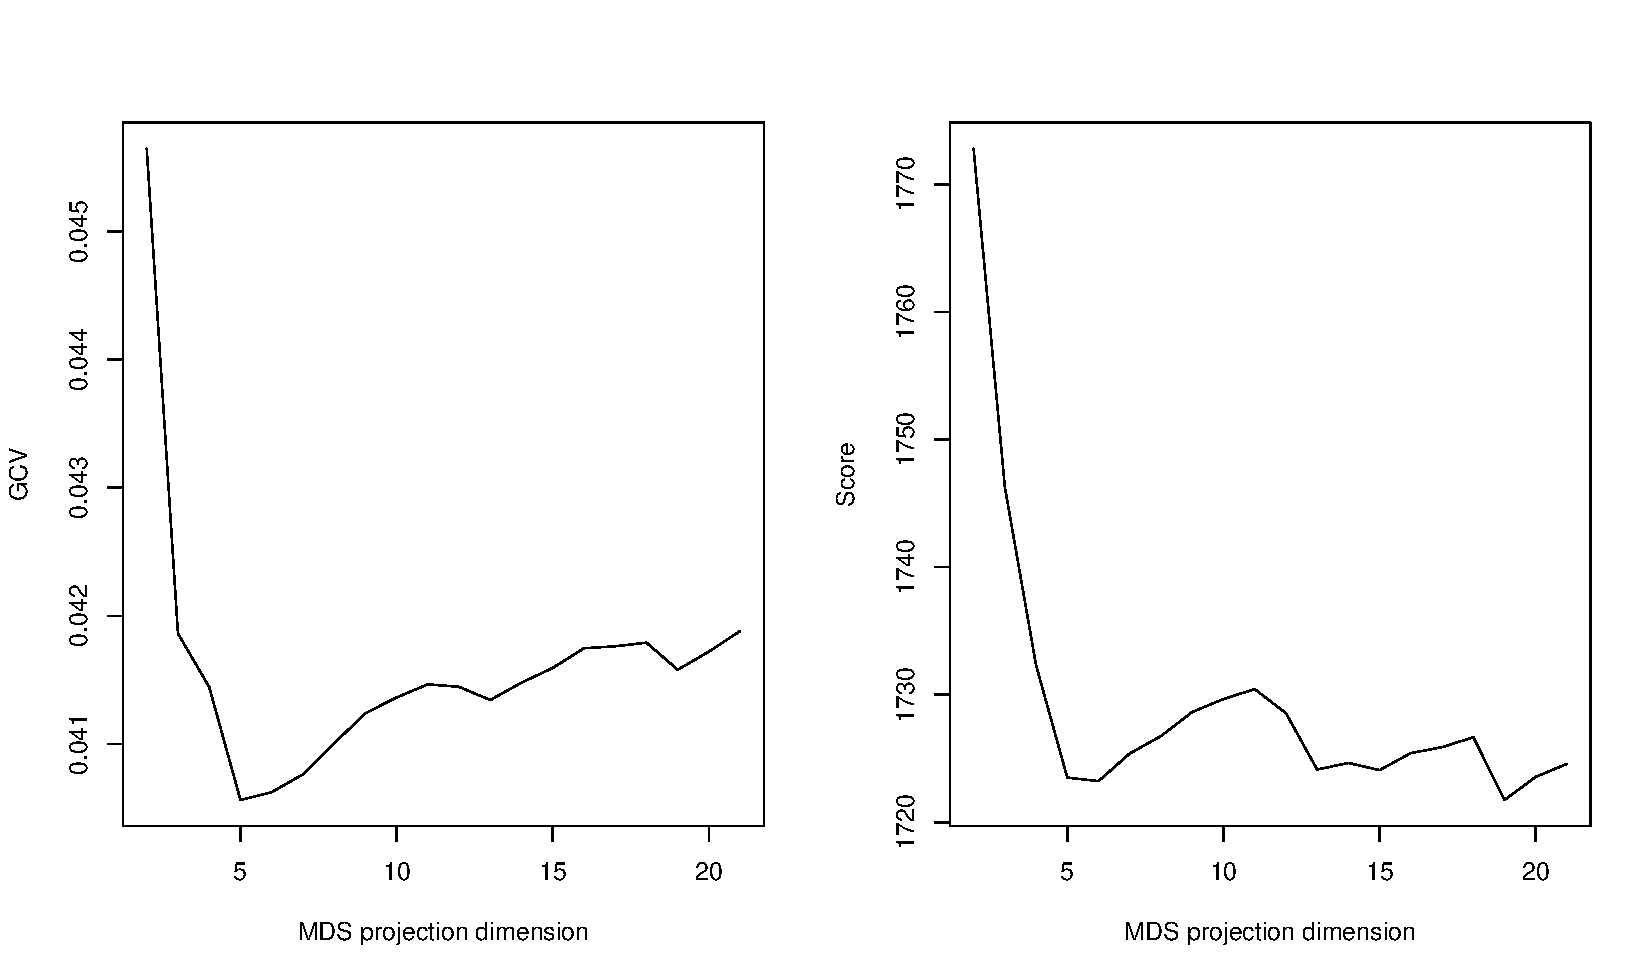
\includegraphics[width=6in]{gds/figs/aral-dim-scores.pdf} \\
\caption{Plots of score against MDS projection dimension for the Aral sea data when GCV (left) and $\text{ML}_p$ are used for dimension selection.}
\label{gds-aral-dim-select}
% generated by duchon/aral-scoreplots.R
\end{figure}


\section{Generalized distance smoothing}
\label{gds-gds-examples}

Duchon splines are able to smooth in high dimensions without the usual problems that come from such situations. Multidimensional scaling allows the projection of any arbitrary distance matrix into Euclidean space. The combination of these two methods has been sucessful in the within-area distance case above, but also allows for smoothing using any set of distances.

Data are often collected on scales that are not necessarily physically meaningful (for example in psychological studies or attitude surveys) but the data are used as if the scale was absolute in some sense (\cite{cox2007}, \cite{torgerson}). In such cases the distances between the observations may be meaningful but the actual ordinal values may not be.

Taking data which is either already distances or distances calculated from data, the MDS projection can be found and then a smooth over those data can be used to model some response. Situations where \mdsds\ might be useful fall into three classes: 
\begin{enumerate}
\item Those in which distances are intrinsically meaningful, where distances between the subjects in a study represent some obviously meaningful physical quantity (for example geographical distance in kilometers between observations of whales.
\item Those in which the combinations of variables in the MDS configuration are not meaningful physically but come together to give a measure of dissimilarity between subjects. In this case all of the variables could be of the same ``kind'' (for example, a repeated measure like voting) or could be combinations of measurements of different phenomena (similar to constructed indices used by econometricians from a series of socio-economic variables (household income, education, state benefits, etc)).
\item Finally, similar to the above class, situations where there are too many variables to be reasonably used in a conventional additive model and therefore using MDS could be used as a variable ``reduction'' technique similar to principle components regression (\cite{elements}, p. 79--80).
\end{enumerate}
The latter two situations pose two interrelated problems. First is that of measurement error: if there are large errors in the variables which are used in the MDS projection, these could unduly influence the result (we usually assume that geographical locations are accurate). For example if there is one very large (erroneous) observation in one of the variables, this could dominate the eigenvalues and cause the variable to have undue prominence in the MDS projection. A thorough treatment of measurement error in non-linear models is given in \cite{measurementerror}. Second is the issue of variable selection; since all variables are used in finding the distances, we have made the assumption that they all affect the response in some way and that the degree to which they have an effect is somehow related to the degree of their variation (or rather, their contribution to the eigenvalues). This is, of course, an unfounded assumption.

All that can be hoped for is that a combination of appropriate distance metric, projection dimension selection and usual model checking will work around the above issues.

\subsection{Examples}

Data where distances between observations are meaningful can come from many different disciplines. Here two examples are given, one from political science and one from biology, however the choice of data here does not indicate any limitation of fields of study to which \mdsds\ can be applied, any discipline in which distances can be measured or calculated \textit{a posteriori} may well benefit from this approach.


\subsubsection{MP data}


The website Public Whip (\url{http://www.publicwhip.org.uk/}) provide data from the Hansard on the votes of 676 MPs in the 1997--2001 Westminster parliament. During this time the House took 1273 divisions. Each vote is coded according to table \ref{voting-code}. Also available from Public Whip are the party allegiances of each MP. 

\begin{table}  
\begin{centering}
\begin{tabular}{ccc}
    Value & Description & Code \\ 
    \hline
    Missing & MP did not vote in this division & 0 \\ 
    Tell aye & MP voted for the motion and was a teller & 1 \\ 
    Aye & MP voted for the motion & 1 \\ 
    Both & MP voted both for  and against the motion & 0 \\ 
    No & MP voted against the motion & -1 \\ 
    Tell no & MP voted against the motion and was a teller & -1 \\ 
  \end{tabular}
\caption{Coding of UK MP voting data. For the purposes of the analysis here the teller's votes are counted as if they voted since we are interested in how voting can be used to predict part affiliation. Note that ``both'' is perfectly possible, and occurs when the MP walks through both the ``Aye'' and ``No'' gates, this can correspond to the MP abstaining (as with ``Missing'') or no nullify a mis-cast vote.}
\end{centering}
\label{voting-code}
\end{table}

Taking the matrix of votes, Euclidean distances between the MPs (rows) were found and used to form the distance matrix. Multidimensional scaling was then used to project these distances into MDS space (dimension selection was performed by optimizing the GCV or $\text{ML}_p$ score). The party affiliation (simplified to Labour party versus not Labour party) was then predicted using a logit link.

Of the 1273 divisions in the 1997--2001 parliament, 17 of them were declared  as ``free votes'' (\cite{freevotes}), where MPs are not ``whipped'' (pressured to take the party line). Predicting affiliation based on whipped votes is relatively easy since MPs are likely to vote along party lines (since they presumably want to keep their leaders happy). Using free votes makes the classification much more difficult. The free votes are summarised in table \ref{free-vote-description}; most of these are ``conscience'' votes.

\begin{table}  
\begin{centering}
\begin{tabular}{cc}
	Date & Bill name \\
    \hline
22 March 2001    &   Election of a Speaker \\
17 January 2001  &   Hunting Bill \\
17 January 2001  &   Hunting Bill \\
17 January 2001  &   Hunting Bill\\
20 December 2000 &   Hunting Bill \\
19 December 2000 &   Human Fertilisation and Embryology\\
31 October 2000  &   Stem Cell Research \\
14 April 2000    &   Medical Treatment (Prevention of Euthanasia) Bill \\
28 February 2000 &   Sexual Offences (Amendment) Bill \\
10 February 2000 &   Sexual Offences (Amendment) Bill \\
28 January 2000  &   Medical Treatment (Prevention of Euthanasia) Bill\\
25 January 1999  &   Sexual Offences (Amendment) Bill\\
22 June 1998     &  Crime and Disorder Bill \\
22 June 1998     &  Crime and Disorder Bill \\
28 November 1997 &  Wild Mammals (Hunting with Dogs) Bill\\
  \end{tabular}
\caption{Free votes in the 1997-2001 parliament (see \cite{freevotes}).}
\end{centering}
\label{free-vote-description}
\end{table}

Using these votes, MPs were selected at random, the model fit to the data and the party affiliation was predicted for those MPs not in the sample. This was repeated for 200 realisations with sample sizes of 200, 300, 400 and 500.

The usual approach for such problems would be to use either a linear model or a variation on the linear model such as the lasso (\cite{elements} pp. 68--69) with a logistic link function. The built-in function \texttt{glm()} is suitable in the first case and the \textsf{R} package \texttt{glmnet} provides a lasso implementation for the latter.

\textbf{SIMON}: Need to add more detail on the lasso?

The four models tested were:
\begin{enumerate}
	\item \mdsds\ (GCV): MDS projection of the data, selected by minimum GCV score over the full range of 2 to the number of dimensions that account for 85\% of the variation in the sample. Spline basis size maximum was 100.
	\item \mdsds\: ($\text{ML}_p$): as previous model but using $\text{ML}_p$ score to select the MDS projection dimension.
	\item Lasso: as implemented in \texttt{glmnet}, cross-validation (using deviance as a loss function) was used to select amount of shrinkage per realisation.
	\item GLM: as implemented in \texttt{glm()}.
\end{enumerate}
For all models the error distribution was binomial and a logit link was used.

To compare the results two metrics were used. First the MSE, as defined in section \ref{DEFN-MSE} and second the Brier score (\cite{brier50}). The Brier score is defined as:
\begin{equation}
\text{BS} = \frac{1}{N} \sum_{i=1}^N (\hat{f}_p(\mathbf{x})-y_i)^2
\end{equation}
where subscript $p$ indicates the probability, rather than the prediction on the response scale. The Brier score therefore has the advantage of offering a more granular measure of the accuracy of a method.

\begin{figure}
\centering
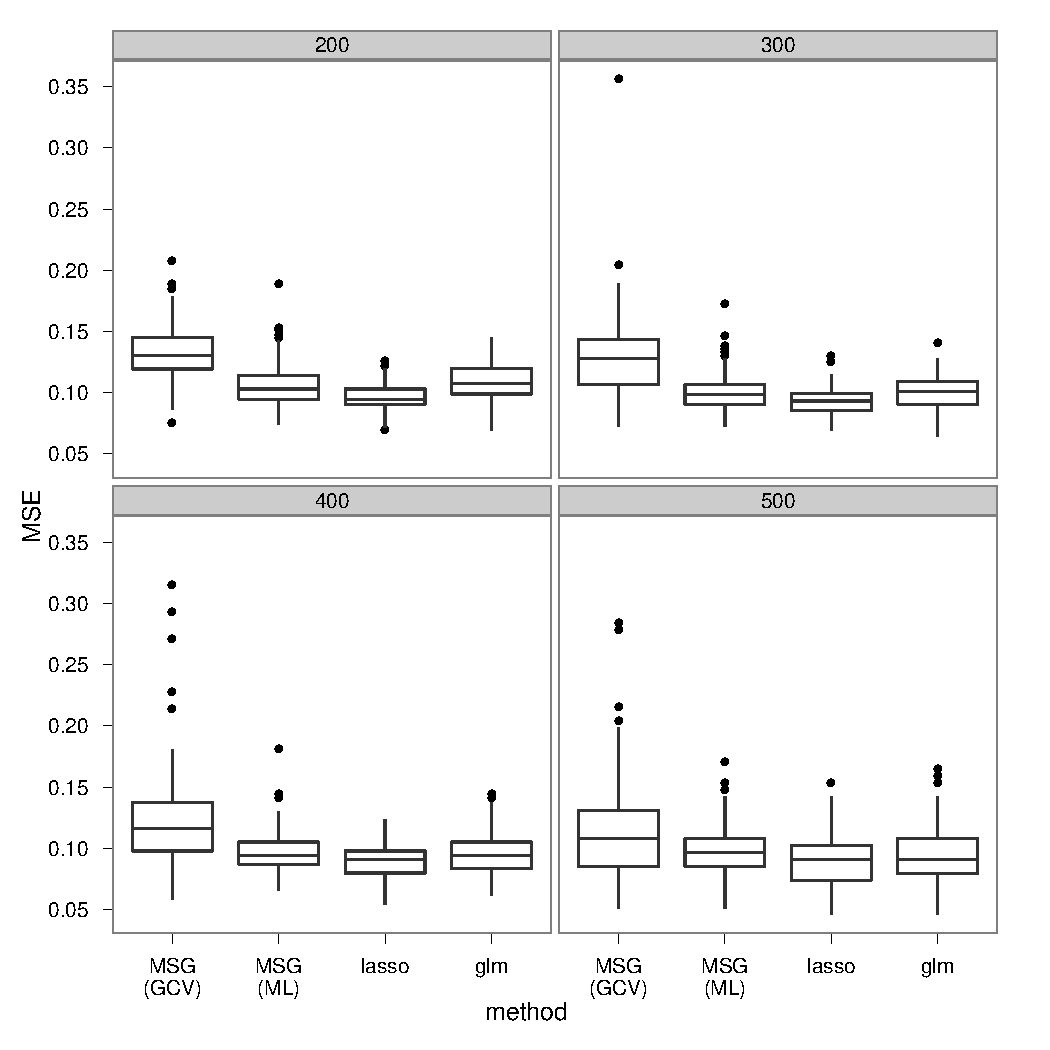
\includegraphics[width=6in]{gds/figs/mp-mse.pdf} \\
\caption{Boxpot of MSE per model for the free vote data set at varying sample sizes.}
\label{gds-mps-mse}
% generated by duchon/mps/analyse-mps.R
\end{figure}

\begin{figure}
\centering
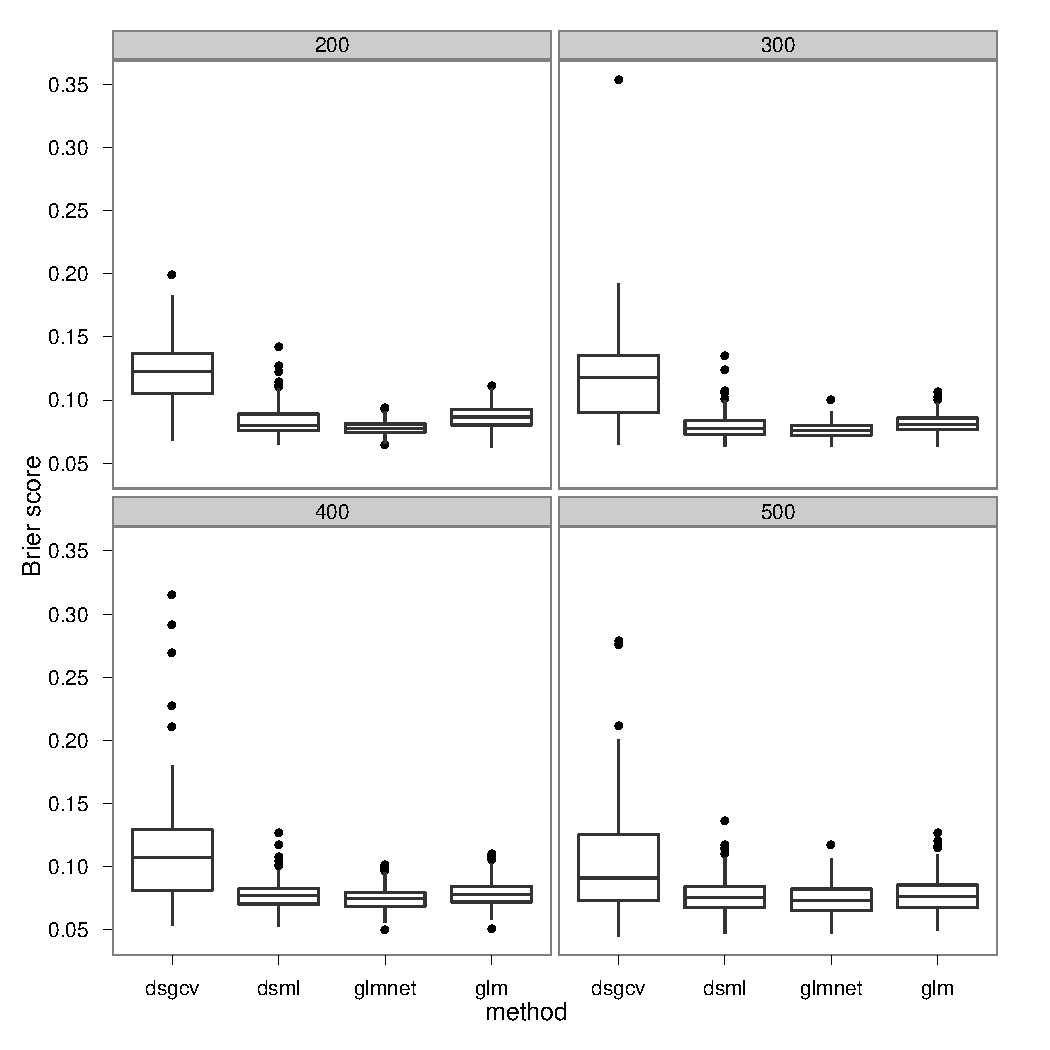
\includegraphics[width=6in]{gds/figs/mp-brier.pdf} \\
\caption{Boxplot of Brier score per model for the free vote data set at varying sample sizes.}
\label{gds-mps-brier}
% generated by duchon/mps/analyse-mps.R
\end{figure}

Figures \ref{gds-mps-mse} and \ref{gds-mps-brier} show boxplots of the MSE and Brier scores respectively at the varying sample sizes. The picture painted by the results is consistent across sample sizes, that is that the lasso out-performs other methods.

(TKTKTK see what happens!!)

TKTKTK want to see what the adjusted penalty does !
      also want to see what the score vs. dimension plots look like (with and without score adjustment)


Interestingly, using the ML score rather than the GCV score for the MDS projection dimension yields better results.

How many dimensions?! - plot!


TKTKTK  how many labour MPs   -- 429/678
TKTKTK confounding with Plaid/SDLP etc






\subsubsection{Breast cancer microarrays}

Microarrays consist of small silicone or glass chips on which thousands of strands of RNA (which can be thought of as carrying instructions from DNA about how to create proteins) are stuck. These strands are known as \textit{targets} or \textit{probes}. When RNA from the sample comes into contact with that on the chip \textit{hybridisation} occurs (hydrogen bonds between matching parts). The targets are have a fluorescent die applied to them before hybridisation and can be scanned afterward to quantify the number of strands from the sample which have attached themselves to the chip, this is known as the \textit{expression level}.

\cite{ernstbook} (pp. 7--9) descibe a data set where both microarray (TKTKTK explain not usual setup, using DNA instead!) and non-genetic data were collected on 62 patients with breast cancer. The microarray contains expression data on 59 genes. Among the non-genetic data collected was the Nottingham Prognostic Index (NPI) (\cite{Haybittle1982} and \cite{Todd1987}), thought to be a good general measure of prognosis for patients with primary breast cancer (ie. cancer that has not spread beyond the breast). The NPI combines 3 pieces of information in a simple equation
\begin{equation}
\text{NPI} = 0.2(\text{size of index lesion in cm}) + \text{number of lymph nodes} + \text{tumour grade}.
\end{equation}
Further information can be found in the references above; it suffices to say that high values of NPI are bad, identifying those patients with very poor prognoses.

\cite{ernstbook} (pp. 240-245) attempt to predict survival based on microarray data, controlling for other factors. Instead here the NPI is to be predicted based on the microarray data. This is not an unreasonable proposal since if one believes that there is some genetic mechanism behind breast cancer (or at least an individuals vulnerability/resistance to it) then the factors making up the NPI could be considered proxies. 

\cite{spang2002} propose that rather that considering a large number individual genes, combinations are used. \cite{spang2002} use a singular value decomposition of the microarray data to perform dimension reduction. The quantities resulting being referred to as ``super-genes''. In a similar way, using distances between patients and then considering the MDS projection of microarray data, we can consider ``eigen-genes''.

In section \ref{gds-gds-examples}, above, it was noted that both errors and non-standardised columns in the data matrix can cause issues with MDS since those variables with the greatest degree of variation do not necessarily inform the model the most. One can easily imagine the case in which a completely unrelated gene was measured with huge error and then made up a huge proportion of the first eigenvalue in the decomposition of the distance matrix, this would dominate the projection but contain no information about the prediction (see also \cite{ernstbook} pp. 220-221). To get around this problem, rather than use the Euclidean distance between patients, the Mahalanobis distance (\cite{mahalanobis}) can be used.

The Mahalanobis distance is easily calculated in the following way. If $x_{i.}$ is a single row from the microarray matrix $X$, this represents a single subject. Imagining that subjects are drawn from some multivariate distribution some mean and covariance matrix $\Sigma$, the Mahalanobis distance $D_m$, between subjects $i$ and $j$ is then defined as:
\begin{equation}
D_m = (x_{i.} - x_{j.})^\text{T} \Sigma^{-1} (x_{i.} - x_{j.}),
\end{equation}
where $\Sigma^{-1}$ is replaced with the inverse of the sample covariance matrix of $X$. The calculated distance takes into account that the data may be more variable in some directions than in others. \cite{gentleman2005} suggest using the Mahalanobis distance in a microarray setting.

Plugging the Mahalanobis distance into the MDS procedure produces a projection in the same way as a set of within-area distances or Euclidean distances would.

Of the 62 patients in the study, 45 had non-missing values for NPI and out of the 59 genes in the microarray, 27 did not have missing values. This lead to a vector of 45 NPI measurements and a 62 by 27 matrix for the microarray data. A number of different \mdsds\ models were fitted, with various error distributions. Using standard checks (eg. \texttt{gam.check()} in \texttt{mgcv}, fitting to residuals etc) two were deemed most promising. Those were a model with normal errors and ine using a quasi-likelihood (\cite{quasi}, \cite{wood2008}) with a square root link function and variance proportional to the square of the mean. As above, the lasso was used for comparison.

Since the sample size is rather small, it was not possible to reasonably split the data into training and validation sets as with the MP data. Instead leave-one-out cross-validation (LOOCV) (see section \ref{DEFN-LOOCV}) was used to assess the sensitivity of the models to changes in the data.

%quasi(power(1/2), variance = mu^2)
%lasso= 1.475949 
%ds ML= 1.418823 
%ds GCV= 1.426787 
%
%Normal
%lasso= 1.421593 
%ds ML= 1.425892 
%ds GCV= 1.410288 


%\subsubsection{Leukemia microarrays}



\section{Software implementation - \mdspack}

The methods detailed in this section, namely the use of Duchon splines along with MDS to perform smoothing are provided in the \textsf{R} package \mdspack\ which is available at\ldots



\section{Conclusion}

TKTKTK sum up, say what else could be done. Show path SC->MDS+RS->MSG, improvements along the way.

